% Generated by TikzMakie.jl. Requires \usepackage{tikz} (and graphicx if images are used).
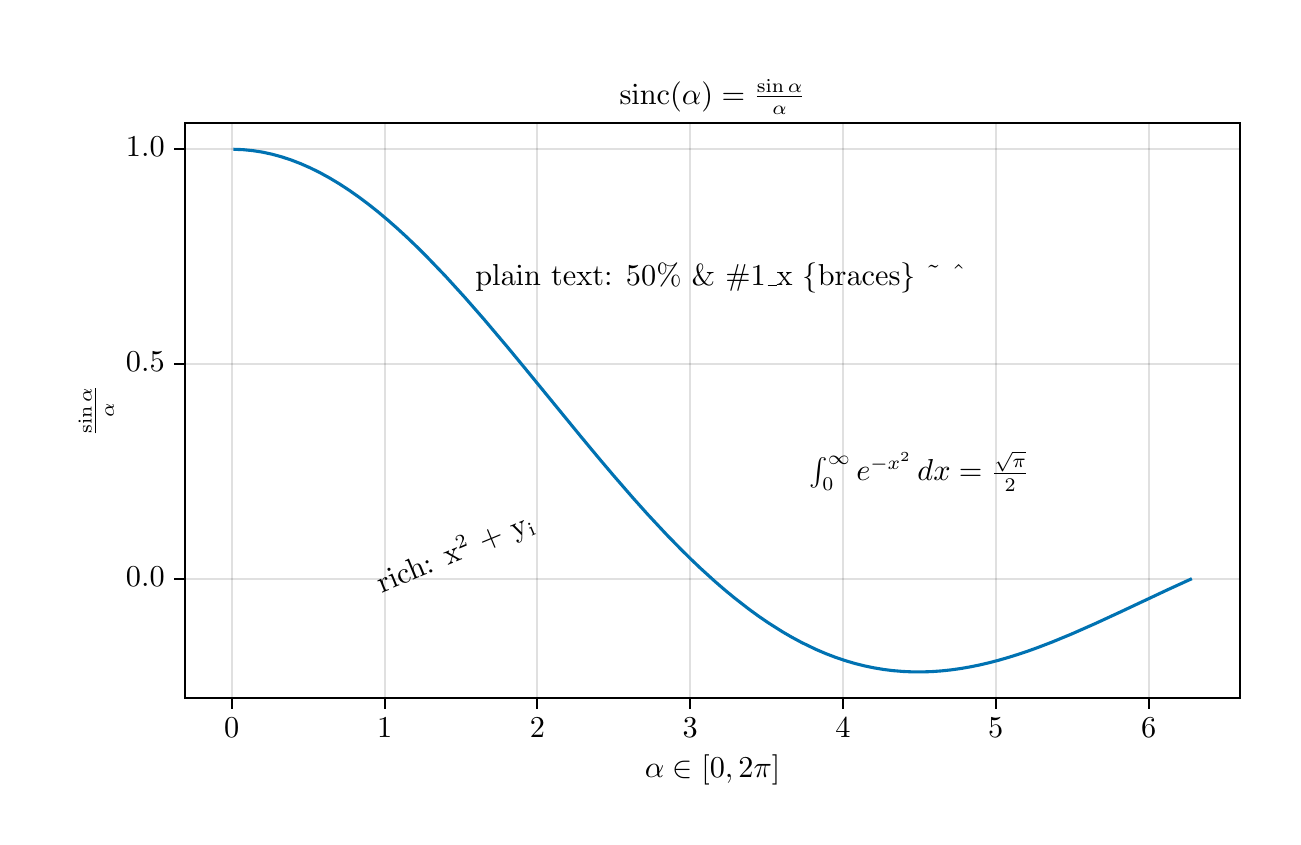
\begin{tikzpicture}[x=0.75pt, y=0.75pt, mknode/.style={inner sep=0pt, outer sep=0pt, execute at begin node={\vphantom{(}}, font=\fontsize{10.5}{12.6}\selectfont}, mkimg/.style={inner sep=0pt, outer sep=0pt}]
\definecolor{mkc1}{RGB}{0,114,178}
\path[use as bounding box] (0,0) rectangle (600,380);
\path[fill=white] (76,57) -- (584,57) -- (584,334) -- (76,334) -- cycle;
\draw[draw=black, line width=0.75pt, draw opacity=0.12]
  (98.35,57) -- (98.35,334)
  (171.97,57) -- (171.97,334)
  (245.59,57) -- (245.59,334)
  (319.21,57) -- (319.21,334)
  (392.83,57) -- (392.83,334)
  (466.44,57) -- (466.44,334)
  (540.06,57) -- (540.06,334);
\draw[draw=black, line width=0.75pt, draw opacity=0.12]
  (76,114.53) -- (584,114.53)
  (76,217.97) -- (584,217.97)
  (76,321.41) -- (584,321.41);
\node[mknode, anchor=north] at (330,29.69) {$\alpha \in [0, 2\pi]$};
\node[mknode, anchor=north] at (98.35,49) {$0$};
\node[mknode, anchor=north] at (171.97,49) {$1$};
\node[mknode, anchor=north] at (245.59,49) {$2$};
\node[mknode, anchor=north] at (319.21,49) {$3$};
\node[mknode, anchor=north] at (392.83,49) {$4$};
\node[mknode, anchor=north] at (466.44,49) {$5$};
\node[mknode, anchor=north] at (540.06,49) {$6$};
\node[mknode, anchor=south, rotate=90] at (41.54,195.5) {$\frac{\sin \alpha}{\alpha}$};
\node[mknode, anchor=east] at (66,114.53) {$0.0$};
\node[mknode, anchor=east] at (66,217.97) {$0.5$};
\node[mknode, anchor=east] at (66,321.41) {$1.0$};
\node[mknode, anchor=south, font=\fontsize{10.5}{12.6}\selectfont\bfseries] at (330,338) {$\mathrm{sinc}(\alpha) = \frac{\sin \alpha}{\alpha}$};
\begin{scope}
\clip (76,57) rectangle (584,334);
\draw[draw=mkc1, line width=1.12pt, miter limit=2]
  (99.09,321.41) -- (103.73,321.23) -- (108.37,320.77) -- (113.02,320.05) -- (117.66,319.05) -- (122.3,317.78)
  -- (126.94,316.25) -- (131.58,314.46) -- (136.22,312.41) -- (140.86,310.11) -- (145.5,307.56) -- (150.15,304.76)
  -- (154.79,301.74) -- (159.43,298.48) -- (164.07,295.01) -- (168.71,291.33) -- (173.35,287.44) -- (177.99,283.36)
  -- (182.64,279.09) -- (187.28,274.65) -- (191.92,270.05) -- (201.2,260.39) -- (210.48,250.2) -- (219.77,239.59)
  -- (231.37,225.86) -- (240.65,214.62) -- (266.18,183.42) -- (275.46,172.25) -- (282.43,164.03) -- (291.71,153.34)
  -- (298.67,145.57) -- (307.95,135.62) -- (314.92,128.5) -- (319.56,123.92) -- (324.2,119.5) -- (331.16,113.17)
  -- (335.8,109.16) -- (340.44,105.33) -- (347.41,99.91) -- (352.05,96.53) -- (356.69,93.35) -- (363.65,88.94)
  -- (368.29,86.25) -- (372.93,83.76) -- (379.89,80.4) -- (384.54,78.42) -- (389.18,76.64) -- (393.82,75.07)
  -- (398.46,73.7) -- (403.1,72.53) -- (407.74,71.56) -- (412.38,70.79) -- (417.03,70.21) -- (421.67,69.83)
  -- (426.31,69.62) -- (430.95,69.6) -- (435.59,69.76) -- (440.23,70.09) -- (444.87,70.58) -- (449.52,71.23)
  -- (454.16,72.04) -- (458.8,72.99) -- (463.44,74.08) -- (468.08,75.3) -- (472.72,76.65) -- (477.36,78.11)
  -- (482.01,79.67) -- (486.65,81.34) -- (493.61,84.01) -- (502.89,87.84) -- (514.5,92.96) -- (526.1,98.32)
  -- (549.31,109.23) -- (560.91,114.53);
\node[mknode, anchor=center] at (333.93,259.35) {plain text: 50\% \& \#1\_x \{braces\} \textasciitilde{} \textasciicircum{}};
\node[mknode, anchor=south west, rotate=22.5] at (171.97,104.19) {rich: x\textsuperscript{2} + y\textsubscript{i}};
\node[mknode, anchor=center] at (429.63,166.25) {$\int_0^\infty e^{-x^2}\,dx = \frac{\sqrt{\pi}}{2}$};
\end{scope}
\draw[draw=black, line width=0.75pt]
  (98.35,56.5) -- (98.35,51.5)
  (171.97,56.5) -- (171.97,51.5)
  (245.59,56.5) -- (245.59,51.5)
  (319.21,56.5) -- (319.21,51.5)
  (392.83,56.5) -- (392.83,51.5)
  (466.44,56.5) -- (466.44,51.5)
  (540.06,56.5) -- (540.06,51.5);
\draw[draw=black, line width=0.75pt]
  (75.5,114.53) -- (70.5,114.53)
  (75.5,217.97) -- (70.5,217.97)
  (75.5,321.41) -- (70.5,321.41);
\draw[draw=black, line width=0.75pt]
  (75.5,57) -- (584.5,57);
\draw[draw=black, line width=0.75pt]
  (76,56.5) -- (76,334.5);
\draw[draw=black, line width=0.75pt]
  (75.5,334) -- (584.5,334);
\draw[draw=black, line width=0.75pt]
  (584,56.5) -- (584,334.5);
\end{tikzpicture}
